\documentclass{ltjsarticle}
\RequirePackage{luatex85}
\usepackage[utf8]{inputenc}
\usepackage[dvipdfmx]{color}
\usepackage{enumerate}
\usepackage{here}
\usepackage{amsthm}
\usepackage{amsfonts}
\usepackage{amsmath}
\usepackage{amssymb}
\usepackage{latexsym}
\usepackage{ytableau}
\usepackage{docmute}
\usepackage{mathtools}
\usepackage{xr}
\usepackage{tikz}
\usetikzlibrary{intersections, calc, arrows.meta}
\usepackage[all]{xy}
\usepackage{graphics}
\usepackage[luatex]{hyperref}
%\usepackage{pxjahyper}



\theoremstyle{definition}
\newtheorem{defin}{定義}[subsection]
\newtheorem{theo}[defin]{定理}
\newtheorem{cor}[defin]{系}
\newtheorem{prop}[defin]{命題}
\newtheorem{lemm}[defin]{補題}
\newtheorem{notice}[defin]{注意}
\newtheorem{eg}[defin]{例}
\newtheorem{fact}[defin]{事実}


\renewcommand{\labelenumi}{(\roman{enumi})}


\newcommand{\invlimit}{\mathop{\lim_{\longleftarrow}}}
\newcommand{\dirlimit}{\mathop{\lim_{\longrightarrow}}}
\newcommand{\ind}{\text{Ind}}
\newcommand{\Hom}{\text{Hom}}
\newcommand{\tr}{\text{tr}}
\newcommand{\id}[1]{\text{id}_{#1}}
\newcommand{\sgn}{\mathrm{sgn}}
\newcommand{\res}[1]{\text{Res}_{#1}}
\newcommand{\generated}[1]{\langle\:#1\:\rangle}
\newcommand{\im}{\text{Im }}
\newcommand{\rank}{\text{rank }}
\newcommand{\del}[2]{\frac{\partial #1}{\partial #2}}
\newcommand{\delsametwo}[2]{\frac{\partial^2 #1}{\partial #2^2}}
\newcommand{\delothertwo}[3]{\frac{\partial^2#1}{\partial#2\partial#3}}
\newcommand{\ddel}[2]{\frac{\partial}{\partial #2}#1}
\newcommand{\ddelsametwo}[3]{\frac{\partial^2}{\partial #2^2}#1}
\newcommand{\ddelothertwo}[3]{\frac{\partial^2}{\partial#2\partial#3}#1}
\newcommand{\simneq}{\not\simeq}
\newcommand{\transpose}[1]{^t\!#1}
\newcommand{\ie}{\text{i.e.}}
\newcommand{\inv}[1]{#1^{-1}}
\newcommand{\real}{\mathbb{R}}
\newcommand{\complex}{\mathbb{C}}
\newcommand{\integer}{\mathbb{Z}}
\newcommand{\quotient}{\mathbb{Q}}
\newcommand{\natnum}{\mathbb{N}}
\newcommand{\proj}{\mathbb{P}}
\newcommand{\affine}{\mathbb{A}}
\newcommand{\tensor}[3]{#1\otimes_#2#3}
\newcommand{\map}[3]{#1:#2\rightarrow#3}
\newcommand{\aut}[2]{\mathrm{Aut}_{#1} (#2)}
\newcommand{\hommoph}[2]{\mathrm{Hom}_{#1}(#2)}
\newcommand{\gl}{\text{GL}}
\newcommand{\End}{\text{End}}
\newcommand{\set}[2]{\left\{\:#1\:\middle|\:#2\:\right\}}
\newcommand{\pmat}[1]{\begin{pmatrix} #1
\end{pmatrix}}
\newcommand{\vmat}[1]{\begin{vmatrix} #1
\end{vmatrix}}
\newcommand{\bmat}[1]{\begin{bmatrix} #1
\end{bmatrix}}
\newcommand{\br}{\vskip\baselineskip}
\newcommand{\Lie}{\text{Lie}}
\newcommand{\Sym}{\text{Sym}}
\newcommand{\Alt}{\text{Alt}}
\newcommand{\ch}{\text{ch}}
\newcommand{\diag}{\text{diag}}
\newcommand{\comb}[2]{_{#1}C_{#2}}
\newcommand{\codim}{\text{codim}\:}
\newcommand{\yd}[1]{\ydiagram{#1}}

\title{aaa}
\author{}
\date{}


\begin{document}
\maketitle

\begin{center}
  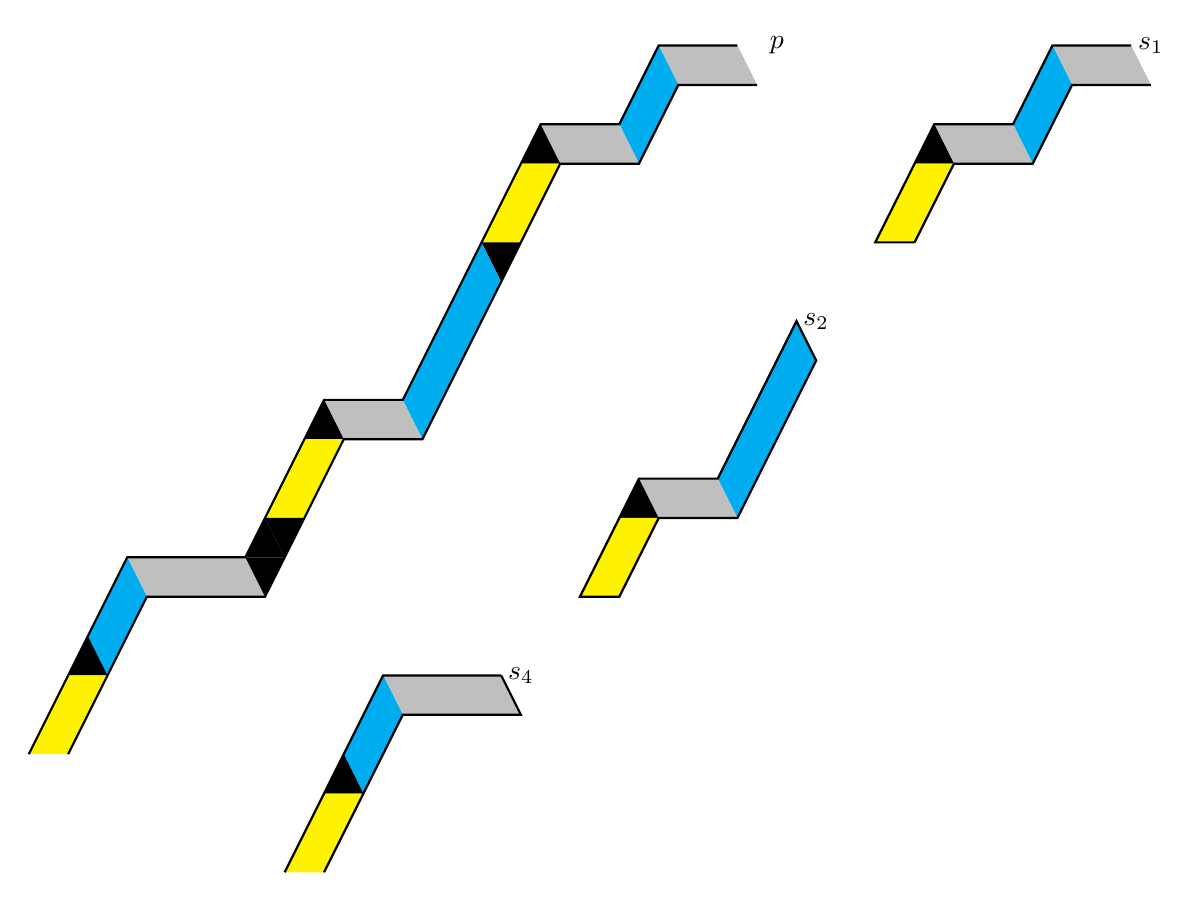
\begin{tikzpicture}


    \node at (8+16/4,16-14/2) {$p$};
    \fill[lightgray] (8+14/4,16-14/2)-- ++(-1,0)-- ++(1/4,-1/2)-- ++(1,0)--cycle;
    \fill[cyan] (8+10/4,16-14/2)-- ++(-1/2,-1)-- ++(1/4,-1/2)-- ++(1/2,1)--cycle;
    \fill[lightgray] (8+8/4,16-16/2)-- ++(-1,0)-- ++(1/4,-1/2)-- ++(1,0)--cycle;
    \fill[black] (8+4/4, 16-16/2)-- ++(-1/4,-1/2)-- ++(1/2,0)--cycle;
    \fill[yellow] (8+3/4, 16-17/2)-- ++(-1/2,-1)-- ++(1/2,0)-- ++(1/2,1)--cycle;
    \fill[black] (8+1/4,16-19/2)-- ++(1/2,0)-- ++(-1/4,-1/2)--cycle;
    \fill[cyan] (8+1/4,16-19/2)-- ++(-1,-2)-- ++(1/4,-1/2)-- ++(1,2)--cycle;
    \fill[lightgray] (8-3/4,16-23/2)-- ++(-1,0)-- ++(1/4,-1/2)-- ++(1,0)--cycle;
    \fill[black] (8-7/4,16-23/2)-- ++(-1/4,-1/2)-- ++(1/2,0)--cycle;
    \fill[yellow] (8-8/4,16-24/2)-- ++(-1/2,-1)-- ++(1/2,0)-- ++(1/2,1)--cycle;
    \fill[black] (8-10/4,16-26/2)-- ++(1/2,0)-- ++(-1/4,-1/2)--cycle;
    \fill[lightgray] (8-11/4,16-27/2)-- ++(-3/2,0)-- ++(1/4,-1/2)-- ++(3/2,0)--cycle;
    \fill[black] (8-10/4,16-26/2)-- ++(-1/4,-1/2)-- ++(1/2,0)--cycle;
    \fill[black] (8-9/4,16-27/2)-- ++(-1/2,0)-- ++(1/4,-1/2)--cycle;
    \fill[cyan] (8-17/4,16-27/2)-- ++(-2/4,-2/2)-- ++(1/4,-1/2)-- ++(2/4,2/2)--cycle;
    \fill[black] (8-19/4,16-29/2)-- ++(-1/4,-1/2)-- ++(1/2,0)--cycle;
    \fill[yellow] (8-20/4,16-30/2)-- ++(-1/2,-1)-- ++(1/2,0)-- ++(1/2,1)--cycle;


    \draw[thick] (8+14/4,16-14/2)-- ++(-1,0)-- ++(-1/2,-1)-- ++(-1,0)-- ++(-7/4,-7/2)-- ++(-1,0)-- ++(-4/4,-4/2)-- ++(-3/2,0)-- ++(-5/4,-5/2);
    \draw[thick] (8+15/4, 16-15/2)-- ++(-1,0)-- ++(-1/2,-1)-- ++(-1,0)-- ++(-7/4,-7/2)-- ++(-1,0)-- ++(-4/4,-4/2)-- ++(-3/2,0)-- ++(-4/4,-4/2);

    \begin{scope}[xshift=5cm]
    \node at (8+15/4,16-14/2) {$s_1$};
    \fill[lightgray] (8+14/4,16-14/2)-- ++(-1,0)-- ++(1/4,-1/2)-- ++(1,0)--cycle;
    \fill[cyan] (8+10/4,16-14/2)-- ++(-1/2,-1)-- ++(1/4,-1/2)-- ++(1/2,1)--cycle;
    \fill[lightgray] (8+8/4,16-16/2)-- ++(-1,0)-- ++(1/4,-1/2)-- ++(1,0)--cycle;
    \fill[black] (8+4/4, 16-16/2)-- ++(-1/4,-1/2)-- ++(1/2,0)--cycle;
    \fill[yellow] (8+3/4, 16-17/2)-- ++(-1/2,-1)-- ++(1/2,0)-- ++(1/2,1)--cycle;
    
    \draw[thick] (8+14/4,16-14/2)-- ++(-1,0)-- ++(-1/2,-1)-- ++(-1,0)-- ++(-3/4,-3/2)-- ++(1/2,0);
    \draw[thick] (8+15/4, 16-15/2)-- ++(-1,0)-- ++(-1/2,-1)-- ++(-1,0)-- ++(-2/4,-2/2);
    \end{scope}

    \begin{scope}[xshift=4cm, yshift=-1cm]
    \node at (8+2/4,16-19/2) {$s_2$};
    \fill[cyan] (8+1/4,16-19/2)-- ++(-1,-2)-- ++(1/4,-1/2)-- ++(1,2)--cycle;
    \fill[lightgray] (8-3/4,16-23/2)-- ++(-1,0)-- ++(1/4,-1/2)-- ++(1,0)--cycle;
    \fill[black] (8-7/4,16-23/2)-- ++(-1/4,-1/2)-- ++(1/2,0)--cycle;
    \fill[yellow] (8-8/4,16-24/2)-- ++(-1/2,-1)-- ++(1/2,0)-- ++(1/2,1)--cycle;

    \draw[thick] (8+1/4,16-19/2)-- ++(-1,-2)-- ++(-1,0)-- ++(-3/4,-3/2)-- ++(1/2,0)-- ++(2/4,2/2)-- ++(1,0)-- ++(1,2)--cycle;
    \end{scope}

    \begin{scope}[xshift=3cm, yshift=-2cm]
      \node at(8-9/4,16-26/2) {$s_4$};
      \fill[lightgray] (8-10/4,16-26/2)-- ++(-3/2,0)-- ++(1/4,-1/2)-- ++(3/2,0)--cycle;
    \fill[cyan] (8-16/4,16-26/2)-- ++(-2/4,-2/2)-- ++(1/4,-1/2)-- ++(2/4,2/2)--cycle;
    \fill[black] (8-18/4,16-28/2)-- ++(-1/4,-1/2)-- ++(1/2,0)--cycle;
    \fill[yellow] (8-19/4,16-29/2)-- ++(-1/2,-1)-- ++(1/2,0)-- ++(1/2,1)--cycle;

    \draw[thick] (8-10/4,16-26/2)-- ++(-3/2,0)-- ++(-5/4,-5/2);
    \draw[thick] (8-10/4,16-26/2)-- ++(1/4,-1/2)-- ++(-1.5,0)-- ++(-4/4,-4/2);
    \end{scope}
  \end{tikzpicture}

  figure 2

  path $p$ とそのsegment $s_1,s_2,s_4$,$s_3$は長さ$0$である.
\end{center}

\end{document}